\subsection{Node}
\begin{center}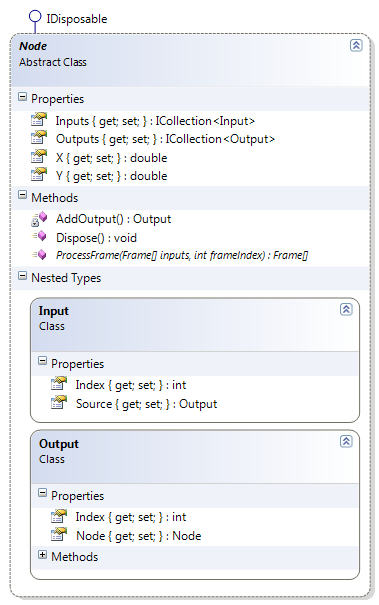
\includegraphics[scale=0.7]{YuvKA.Pipeline/node.png} \\
\end{center}
Die Basisklasse \name{Node} stellt die Attribute und Methoden zur Verfügung, welche von allen Knoten (seien dies Eingabe-, Ausgabe- oder Manipulationsknoten) benötigt werden. Dies umfasst die \name{Process}-Methode, welche die tatsächliche Bearbeitung der \name{Frame}s darstellt, als auch alle Informationen bezüglich der Verbindungen zwischen verschiedenen Knoten, welche in den inneren Klassen \name{Input} und \name{Output} gestellt sind.

\subsubsection{YuvKA.Pipeline.Node}

\begin{verbatim}
[InheritedExport]
[DataContract]
public abstract class Node : IDisposable
\end{verbatim}

\paragraph{Beschreibung}~\\
Die abstrakte Klasse \name{Node} stellt die gemeinsame Struktur aller Knoten zur Verfügung. Die allgemeine Arbeitsweise eines solchen Knotens besteht darin, dass er nach seiner Konstruktion und dem Verbinden seiner Eingänge (falls er welche hat) durch einen Aufruf der Funktion \name{Process} zur Verarbeitung der gegebenen \name{Frame}s ab dem gegebenen Index gebracht wird. Was die Bearbeitung beinhaltet, wird in der jeweiligen Unterklasse spezifiziert.

\paragraph{Typmember}
\begin{itemize}

\property{X}
	\begin{verbatim}
	[Browsable(false)]
	[DataMember]
	public double X { get; set; }
	\end{verbatim}
	Stellt die X-Koordinate des Knoten im Graphen dar.

\property{Y}
	\begin{verbatim}
	[Browsable(false)]
	[DataMember]
	public double Y { get; set; }
	\end{verbatim}
	Stellt die Y-Koordinate des Knoten im Graphen dar.

\property{Inputs}
	\begin{verbatim}
[Browsable(false)]
public ICollection<Input> Inputs { get; private set; }
	\end{verbatim}
Stellt die Eingänge eines Knoten dar. Siehe innere Klasse \name{Input}.

\property{Outputs}
	\begin{verbatim}
[Browsable(false)]
public ICollection<Output> Outputs { get; private set; }
	\end{verbatim}
Stellt die Ausgänge eines Knoten dar. Siehe innere Klasse \name{Output}.

\method{Process}
	\begin{verbatim}
public abstract Frame[] Process(Frame[] inputs, int tick);
	\end{verbatim}
	Verarbeitet die gegebenen \name{Frame}s entsprechend dem internen Algorithmus und gibt ein Array von \name{Frame}s als Resultat zurück. Der Parameter \name{inputs} ist hierbei direkt als die Daten, welche an den Eingängen des Knotens anliegen, zu interpretieren. Dementsprechend entspricht der Rückgabewert den Daten, welche an den Ausgängen des Knotens durchgereicht werden. Verschiedene Knoten überschreiben diese Methode mit verschiedenen Implementationen.


\end{itemize}

\subsubsection{YuvKA.Pipeline.Node.Input}

\begin{verbatim}
public class Input
\end{verbatim}

\paragraph{Beschreibung}~\\
Die innere Klasse \name{Input} stellt einen Eingang eines Knotens dar, von dem der Knoten seine zu verarbeitenden Daten bezieht. \footnote{Dies gilt natürlich nicht für Unterklassen der Klasse \name{InputNode}, welche in der Regel keine Eingänge haben und ihre Daten von anderen Stellen beziehen.}

\paragraph{Typmember}
\begin{itemize}

\property{Source}
	\begin{verbatim}
public Output Source { get; set; }
	\end{verbatim}
Enthält die Quelle des Einganges. Graphisch gesehen entspricht dies dem ``Anfang der Kante'' zwischen zwei Knoten.

\property{Index}
	\begin{verbatim}
public int Index { get; }
	\end{verbatim}
Speichert den Index des Einganges. Dies ist insbesondere bei Knoten wichtig, welche einen Unterschied zwischen verschiedenen Eingängen machen. \footnote{Beispiel: Der \name{DifferenceNode}-Knoten, welcher die Pixeldaten verschiedener Eingänge voneinander subtrahiert.}

\end{itemize}


\subsubsection{YuvKA.Pipeline.Node.Output}

\begin{verbatim}
public class Input
\end{verbatim}

\paragraph{Beschreibung}~\\
Die innere Klasse \name{Output} stellt einen Ausgang eines Knotens dar, durch den die verarbeiteten Daten eines Rechenschrittes weitergegeben werden. \footnote{Dies gilt natürlich nicht für Unterklassen der Klasse \name{OutputNode}, welche in der Regel keine Ausgänge haben.}

\paragraph{Typmember}
\begin{itemize}

\property{Node}
	\begin{verbatim}
public Node Node { get; }
	\end{verbatim}
Speichert den Knoten, zu dem der Ausgang gehört.

\property{Index}
	\begin{verbatim}
public int Index { get; }
	\end{verbatim}
Speichert den Index des Ausgangs. Dies ist insbesondere bei Knoten wichtig, welche einen Unterschied zwischen verschiedenen Ausgängen machen \footnote{Beispiel: Der \name{RgbSplitNode}-Knoten, welcher die Pixeldaten seiner Eingabe in Rot-, Grün- und Blaukanal aufteilt.}

\end{itemize}
